\section{PŘESNÝ DVOUSTUPŇOVÝ OPERAČNÍ ZESILOVAČ}
Základní koncept přesného návrhu zesilovače, vstupní bipolární stupeň, princip eliminace chyby, postup návrhu

\subsection{Základní koncept přesného návrhu zesilovače a eliminace chyby}
Popisuje strategii postupu při návrhu přesného OZ. Tato strategie se dá použít v čadě návrhů u nichž je přesnost prioritou. Přesnost OZ je většinou dána jediným parametrem - velikostí jeho vstupní napěťové nesymetrie $\sigma$vos. Vychází z toho, jakým způsobem se chová operační zesilovač se zpětnou vazbou.

\begin{figure}[h]
   \begin{center}
     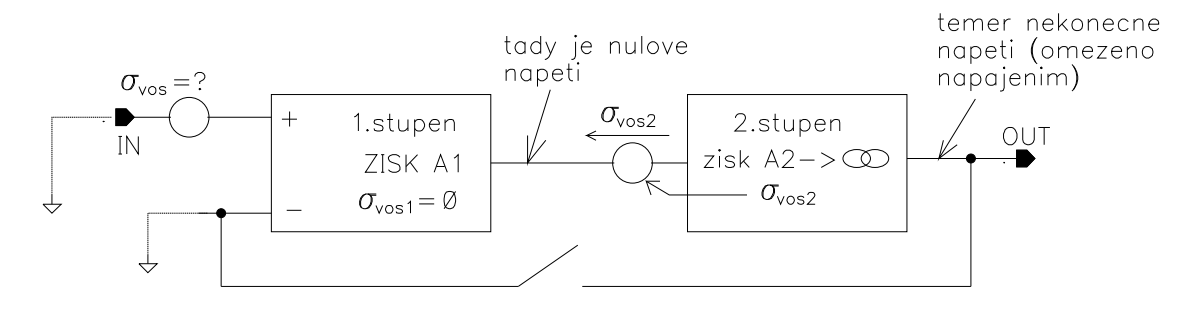
\includegraphics[scale=0.5]{images/dvojOZ.png}
   \end{center}
   \caption{Blokové schéma dvojstupňového zesilovače}
\end{figure}

Předpokládejme, že první stupeň má konečnou hodnotu zisku A1 a je naprosto přesný (jeho offset je nulový). Druhý stupeň má "téměř nekonečný" zisk A2 a hodnotu offsetu $\sigma$vos2. Představme si nyní rozpojenou zpětnou vazbu a uzemněné vstupy. Na výstupu prvního stupně je nulové napětí, jako důsledek $\sigma$vos1. Na vstupu druhého stupně je potom napětí jeho nesymetrie $\sigma$vos2. Vzhledem k téměř nekonečnému zisku A2 je potom na výstupu OUT téměř nekonečně kladné napětí (v praxi omezeno Ucc). 

Pokud nyní uzavřeme zpětnou vazbu, dostane se výstupní (kladné) napětí na invertující vstup. To má za následek pokles výstupního napětí prvního stupně do záporných hodnot a tato záporná hodnota výstupního napětí prvního stupně se odečítá s napětím offsetu $\sigma$vos2 dtuhého stupně. Nakonec se celý systém ustálí ve stavu při němž první stupeň generuje napětí, jehož hodnota je stejná jako hodnota $\sigma$vos2, ale má opačnou polaritu. To je možné pouze tak, že jeho vstupní napětí má hodnotu:
\begin{equation}
V_{os} = -\frac{\sigma_{vos2}}{A1}
\end{equation}

\begin{figure}[h]
   \begin{center}
     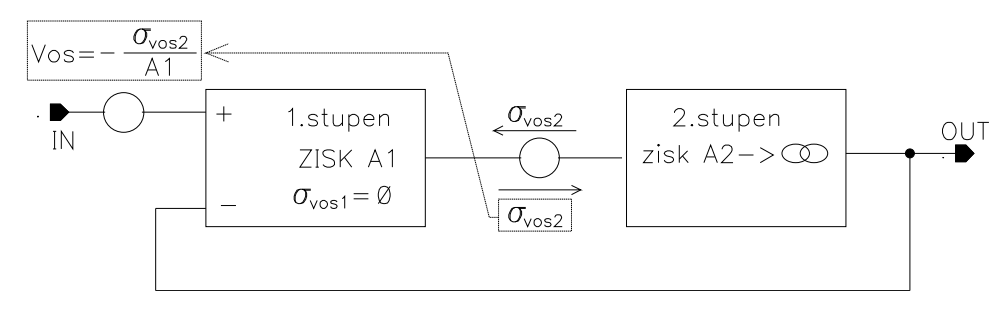
\includegraphics[scale=0.5]{images/dvojOZ2.png}
   \end{center}
   \caption{Blokové schéma dvojstupňového zesilovače-připojená zpětná vazba}
\end{figure}

Stačí tedy navrhnout dostatečně přesný první zesilovací stupeň a tento zesilovací stupeň eliminuje vstupní chybu (offset) následujícího stupně tak, že jej převádí na svůj vstup podělená svým vlastním ziskem A1. Podle velikosti chyby $\sigma$vos2 následujícího stupně se potom nastaví dostatečná (co nejmenší kvůli stabilitě) hodnota zisku A1. Běžným "nejpřesnějším" zesilovacím blokem je bipolární diferenciální zesilovač s odporovou zátěží a to přímo určuje architekturu běžných OZ.

\subsection{Vstupní bipolární stupeň}

\begin{figure}[h]
   \begin{center}
     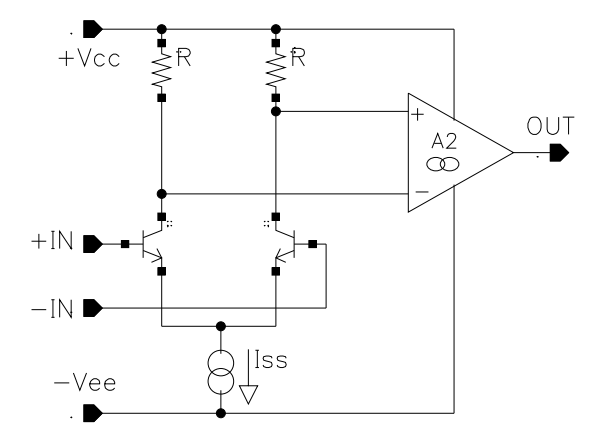
\includegraphics[scale=0.5]{images/prvnistupen.png}
   \end{center}
   \caption{Vstupní bipolární stupeň}
\end{figure}

Transkonduktance gm1:
\begin{equation}
gm_{1} = \frac{I_{ss}}{2*U_{T}}
\end{equation}

Zisk A1:

\begin{equation}
A1 = gm_{1}*R=\frac{I_{ss}*R}{2*U_{T}}
\end{equation}

\newpage
\subsection{Postup návrhu}

První stupeň se navrhne jako přesný diferenciální zesilovač s co nejmenším vstupním offsetem $\sigma$vos1 a s dostatečně velkým ziskem A1. Tento zisk A1 potom eliminuje vliv offsetu $\sigma$vos2 druhého stupně. Opět se používá podmínka:
\begin{equation}
\frac{\sigma_{vos2}}{A1} = \frac{\sigma_{vos1}}{2}
\end{equation}

Vypočítáme hodnotu offsetu $\sigma$vos:
\begin{equation}
\sigma_{vos} = \sqrt{\sigma_{vos1}^2+(\frac{\sigma_{vos2}^2}{A1})^2}\leqslant1,12*\sigma_{vos1}=> \sigma_{vos} \approx \sigma_{vos1}
\end{equation}

Potom vliv offsetu druhého stupně je zanedbatelný. Jako přesný diferenciální stupeň se často používá odporově zatížený NPN stupeň, v běžných procesech má takovýto stupeň nejvyšší dosažitelnou přesnost. Jeho zisk A1 se pro běžné aplikace volí jen takový (nízký), aby stačil dostatečně na potlačení chyby $\sigma$vos2 (vstupního offestu) druhého stupně. Vyšší než nezbytný zisk A1 může přinést problémy se stabilitou. Nevýhodou NPN dif. stupně může být poměrně velký vstupní odpor.

\begin{figure}[h]
   \begin{center}
     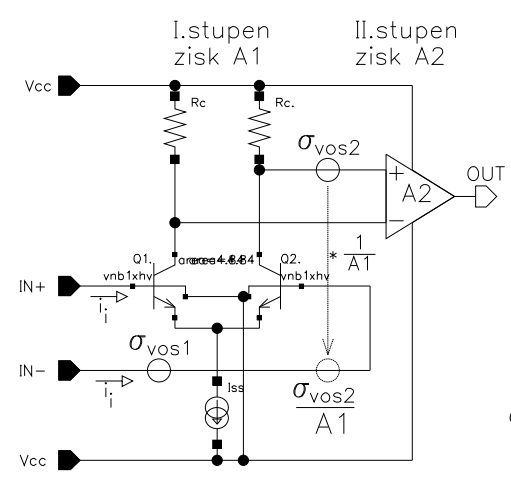
\includegraphics[scale=0.5]{images/OZ.png}
   \end{center}
   \caption{Návrh zesilovače}
\end{figure}

První stupeň má maximální možnou přesnost, která je dána offsetem $\sigma$vos1. Současně má první stupeň dostatečně vysoký zisk A1, který eliminuje vstupní chybu $\sigma$vos2 druhého stupně. Celková přesnost je potom dána pouze offsetem $\sigma$vos1 prvního stupně.

Dalším krokem je výpočet vstupního offsetu $\sigma$vos2 druhého stupně. Ten je dán nekorelovaným součtem chyny $\sigma$vos2 vlastního druhého stupně a chyby $\sigma$vosl sledovače. Chyba sledovače se skládá z chyby $\sigma$voss vlastních tranzistorů sledovače (MAL a MBL) a z chyby $\sigma$vosi nesouběhu jejich proudových zdrojů MSA a MSB.

\begin{figure}[h]
   \begin{center}
     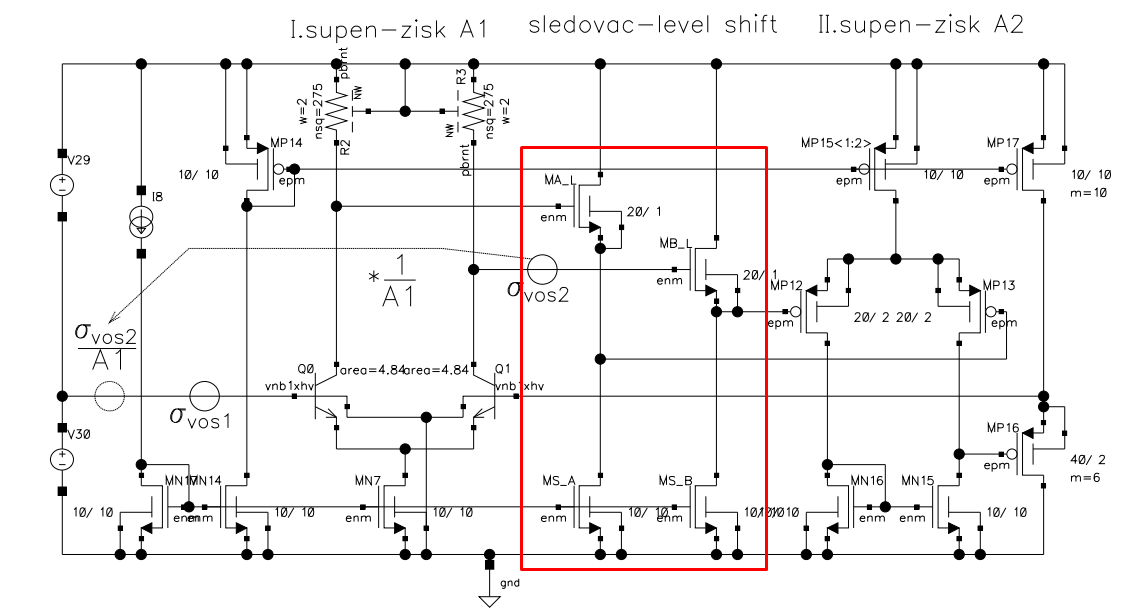
\includegraphics[scale=0.5]{images/sled.png}
   \end{center}
   \caption{Umístění sledovače a jeho proudových zdrojů}
\end{figure}

Celková vstupní chyba $\sigma$vosl sledovače je potom spočítána jako:
\begin{equation}
\sigma_{vosl}=\sqrt{\sigma_{voss}^2+(\frac{\sigma_{voi}}{gms})^2}
\end{equation}
, kde transkonduktance MOS tranzistoru se vypočítá jako:
\begin{equation}
gm = \sqrt{2*I_{d}*kp*\frac{W}{L}}
\end{equation}

Dalším krokem je výpočet offsetu vlastního druhého stupně ($\sigma$vos2). Tato chyba je dána kombinací chyby $\sigma$vo2i diferenciálního stupně a chyby $\sigma$iz souběhu tranzistoru MZ1 a MZ2.

\begin{figure}[h]
   \begin{center}
     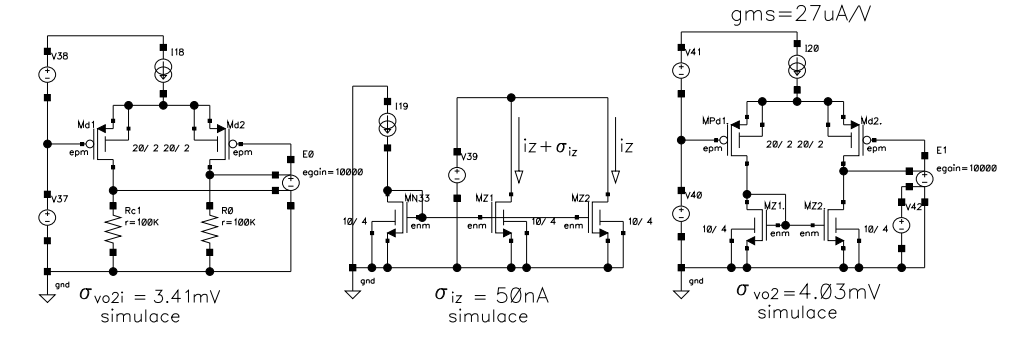
\includegraphics[scale=0.5]{images/offset2.png}
   \end{center}
   \caption{Výpočet offsetu vlastního druhého stupně}
\end{figure}
\pagebreak
Tato chyba se vypočítá:
\begin{equation}
\sigma_{vo2}=\sqrt{\sigma_{vo2i}^2+(\frac{\sigma_{iz}}{gms})^2}
\end{equation}

Nyní můžeme vypočítat celkový vstupní offset $\sigma$vos2 celého druhého stupně (vlastní druhý stupeň a sledovač) jako nekorelovaný součet chyby $\sigma$vos2 vlastního druhého stupně a chyby $\sigma$vosl sledovače:
\begin{equation}
\sigma_{vos2}=\sqrt{\sigma_{vo2}^2+\sigma_{vosl}^2}
\end{equation}

Posledním krokem je návrh zisku A1 prvního stupně. Tento stupěň má chybu $\sigma$vos1. Druhý stupeň má chybu (offset) $\sigma$vos2. Tato chyba je eliminována ziskem A1 - pro zanedbání offsetu $\sigma$vos2 druhého stupně musí platit
\begin{equation}
\frac{\sigma_{vos2}}{A1}\leq\frac{\sigma_{vos1}}{2} => A1\geq2*\frac{\sigma_{vos2}}{\sigma_{vos1}}
\end{equation}

Napěťový zisk A1 odporově zatíženého bipolárního diferenciálního stupně je dán poměrem úbytku na zatěžovacích odporech a teplotního napětí Ut:
\begin{equation}
A1=\frac{I_{c}*R_{c}}{U_{T}} => R_{c}=\frac{A1*U_{T}}{I_{C}}
\end{equation}

Celková hodnota vstupní chyby $\sigma$vos (offsetu) se potom spočítá jako:
\begin{equation}
\sigma_{vos}=\sqrt{\sigma_{vos1}^2+(\frac{\sigma_{vos2}}{A1})^2}
\end{equation}


















